\documentclass{beamer}
\usepackage{amsmath}
\usepackage[english]{babel} %set language; note: after changing this, you need to delete all auxiliary files to recompile
\usepackage[utf8]{inputenc} %define file encoding; latin1 is the other often used option
\usepackage{csquotes} % provides context sensitive quotation facilities
\usepackage{graphicx} %allows for inserting figures
\usepackage{booktabs} % for table formatting without vertical lines
\usepackage{textcomp} % allow for example using the Euro sign with \texteuro
\usepackage{stackengine}
\usepackage{wasysym}
\usepackage{tikzsymbols}
\usepackage{textcomp}
\newcommand{\bubblethis}[2]{
        \tikz[remember picture,baseline]{\node[anchor=base,inner sep=0,outer sep=0]%
        (#1) {\underline{#1}};\node[overlay,cloud callout,callout relative pointer={(0.2cm,-0.7cm)},%
        aspect=2.5,fill=yellow!90] at ($(#1.north)+(-0.5cm,1.6cm)$) {#2};}%
    }%
\tikzset{face/.style={shape=circle,minimum size=4ex,shading=radial,outer sep=0pt,
        inner color=white!50!yellow,outer color= yellow!70!orange}}
%% Some commands to make the code easier
\newcommand{\emoticon}[1][]{%
  \node[face,#1] (emoticon) {};
  %% The eyes are fixed.
  \draw[fill=white] (-1ex,0ex) ..controls (-0.5ex,0.2ex)and(0.5ex,0.2ex)..
        (1ex,0.0ex) ..controls ( 1.5ex,1.5ex)and( 0.2ex,1.7ex)..
        (0ex,0.4ex) ..controls (-0.2ex,1.7ex)and(-1.5ex,1.5ex)..
        (-1ex,0ex)--cycle;}
\newcommand{\pupils}{
  %% standard pupils
  \fill[shift={(0.5ex,0.5ex)},rotate=80] 
       (0,0) ellipse (0.3ex and 0.15ex);
  \fill[shift={(-0.5ex,0.5ex)},rotate=100] 
       (0,0) ellipse (0.3ex and 0.15ex);}

\newcommand{\emoticonname}[1]{
  \node[below=1ex of emoticon,font=\footnotesize,
        minimum width=4cm]{#1};}
\usepackage{scalerel}
\usetikzlibrary{positioning}
\usepackage{xcolor,amssymb}
\newcommand\dangersignb[1][2ex]{%
  \scaleto{\stackengine{0.3pt}{\scalebox{1.1}[.9]{%
  \color{red}$\blacktriangle$}}{\tiny\bfseries !}{O}{c}{F}{F}{L}}{#1}%
}
\newcommand\dangersignw[1][2ex]{%
  \scaleto{\stackengine{0.3pt}{\scalebox{1.1}[.9]{%
  \color{red}$\blacktriangle$}}{\color{white}\tiny\bfseries !}{O}{c}{F}{F}{L}}{#1}%
}
\usepackage{fontawesome} % Social Icons
\usepackage{epstopdf} % allow embedding eps-figures
\usepackage{tikz} % allows drawing figures
\usepackage{amsmath,amssymb,amsthm} %advanced math facilities
\usepackage{lmodern} %uses font that support italic and bold at the same time
\usepackage{hyperref}
\usepackage{tikz}

\usepackage{tcolorbox}

\usefonttheme[onlymath]{serif} %set math font to serif ones

\definecolor{beamerblue}{rgb}{0.2,0.2,0.7} %define beamerblue color for later use

%%% defines highlight command to set text blue
\newcommand{\highlight}[1]{{\color{blue}{#1}}}


%%%%%%% commands defining backup slides so that frame numbering is correct

\newcommand{\backupbegin}{
   \newcounter{framenumberappendix}
   \setcounter{framenumberappendix}{\value{framenumber}}
}
\newcommand{\backupend}{
   \addtocounter{framenumberappendix}{-\value{framenumber}}
   \addtocounter{framenumber}{\value{framenumberappendix}}
}

%%%% end of defining backup slides

%Specify figure caption, see also http://tex.stackexchange.com/questions/155738/caption-package-not-working-with-beamer
\setbeamertemplate{caption}{\insertcaption} %redefines caption to remove label "Figure".
%\setbeamerfont{caption}{size=\scriptsize,shape=\itshape,series=\bfseries} %sets figure  caption bold and italic and makes it smaller


\usetheme{Boadilla}

% --------------------
% Overall information
% --------------------

\title[Economía I]{Economía I \vspace{4mm}
\\ Magistral 14: Distorsiones al equilibrio competitivo}
\date{}
\author[Riottini]{Riottini Franco}
\vspace{0.4cm}
\institute[]{Universidad de San Andrés} 

\begin{document}

\begin{frame}
\titlepage
\centering

\includegraphics[scale=0.2]{../Figures/logoUDESA.jpg} 
\end{frame}

\begin{frame}{Distorsiones al equilibrio de mercado}
    \begin{itemize}
        \item En muchas ocasiones el mercado no funciona tan perfectamente
        \vspace{1mm}
        \item Hay dos tipos de desvíos
        \begin{itemize}
            \item Los creados por el hombre
            \item Los que se imponen por características de la realidad
        \end{itemize}
    \end{itemize}
\end{frame}


\begin{frame}{Distorsiones al equilibrio de mercado}
    \begin{itemize}
        \item Creadas por el hombre:
        \begin{itemize}
            \item Monopolios artificiales (farmacias, escribanos, low cost)
             \vspace{1mm}
            \item Impuestos
             \vspace{1mm}
            \item Precios máximos o mínimos (cepo)
             \vspace{1mm}
            \item Regulación (ley de alquileres)
        \end{itemize}
        \item Por las características de la realidad
        \begin{itemize}
            \item Monopolios naturales (red eléctrica, agua, gas)   
             \vspace{1mm}
            \item Externalidades
             \vspace{1mm}
            \item Bienes públicos
            \vspace{1mm}
            \item Problemas de información
            \begin{itemize}
                \item Atributos ocultos (selección adversa)
                 \vspace{1mm}
                \item Acciones ocultas (moral hazard o riesgo moral)
            \end{itemize}        
        \end{itemize}
    \end{itemize}
\end{frame}

\begin{frame}{El impacto de los impuestos}
    \begin{itemize}
        \item ¿Qué es un impuesto?
        \item Es un tributo generalmente establecido por el Estado
        \begin{itemize}
            \item Para financiar sus gastos
            \item Para ‘guiar’ el comportamiento (por ejemplo en el caso de externalidades)
        \end{itemize}
        \item Existen diversos tipos:
        \begin{itemize}
            \item Al consumo, al trabajo, al ingreso, a la propiedad, etc.
        \end{itemize}
        \item Un impuesto aumentará el precio que los consumidores pagan sobre un bien...
        \item La elasticidad precio de la demanda tendrá influencia sobre el efecto del impuesto
    \end{itemize}
\end{frame}

\begin{frame}{Impuestos y eficiencia}
    \begin{itemize}
        \item La introducción de impuestos aleja la economía del equilibrio competitivo
        \begin{itemize}
            \item Los impuestos sobre oferentes/consumidores ``desplazan" la curva de oferta/demanda porque el precio es más alto para cada cantidad
            \item Al recaudar impuestos el Estado genera una pérdida de peso muerto
        \end{itemize}
        \item La recaudación se extrae del excedente de consumidores y productores
        \begin{itemize}
            \item La incidencia del impuesto depende de la elasticidad relativa de consumidores y productores
            \item El grupo menos elástico lleva más de la carga fiscal
            \item ¿Por qué?
        \end{itemize}
    \end{itemize}
\end{frame}

\begin{frame}{Impacto de un impuesto a los vendedores}
    \centering
    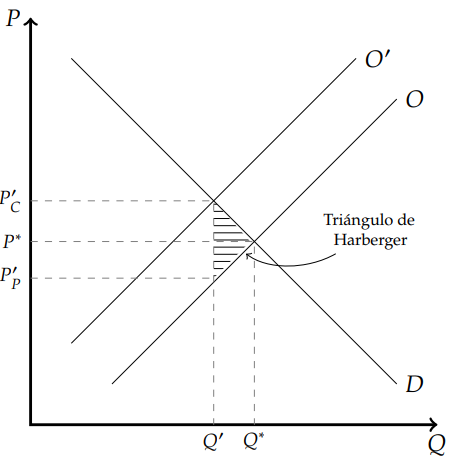
\includegraphics[scale=0.7]{../Figures/C24.1.png}
\end{frame}

\begin{frame}{Impacto de los impuestos}
    \begin{itemize}
        \item ¿Cuánto va a cambiar los impuestos el comportamiento de los individuos?
        \begin{itemize}
            \item ¿Qué tan grande va a ser la pérdida de peso muerto? \\
            - ¿Porqué es relevante conocer la elasticidad de demanda? \\
            - ¿Qué tipo de productos tienen demanda inelástica?
        \end{itemize}
        \item ¿Qué hace el gobierno con los recursos que recauda?
        \item A veces el gobierno quiere cambiar el comportamiento
    \end{itemize}
\end{frame}

\begin{frame}
\frametitle{Impuestos y elasticidad}
\begin{itemize}
    \item Un impuesto puede reducir mucho las ventas si su demanda es altamente elástica
    \begin{itemize}
        \item ¡Y eso puede ser lo que el gobierno intenta hacer! \\
        - Por ej., impuestos sobre bienes ‘malos’ para la sociedad como el tabaco o el alcohol o por contaminar
    \end{itemize}
    \item Pero si un impuesto causa una importante caída en las ventas, también reduce los ingresos del impuesto
    \item Si un gobierno que desea aumentar los ingresos a partir del impuesto, debería elegir gravar productos con demanda inelástica
    \begin{itemize}
        \item ¿Qué tipo de productos pueden tener una demanda de estas características?
    \end{itemize}
\end{itemize}
\end{frame}

\begin{frame}{Impacto de un impuesto a productos inelásticos}
    \centering
    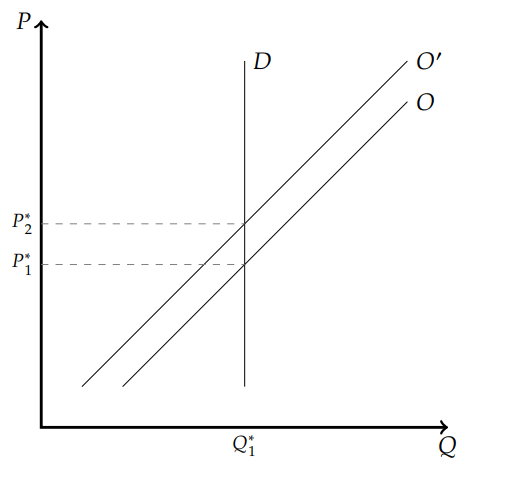
\includegraphics[scale=0.7]{../Figures/C24.3.png}
\end{frame}

\begin{frame}{Distorciones e incidencia}
    \begin{itemize}
        \item Cuanto más inelástica la demanda menor la incidencia impositiva (\textbf{¿Qué pasa si la oferta es inelástica?})
        \item Para demandas con el mismo nivel de elasticidad, mantener la ineficiencia constante implica que tengamos estructuras impositivas similares (IVA).
        \item Impuestos en cascada (IIBB, \textbf{ejemplo numerico?})
        \item ¿Quién paga los impuestos? $\rightarrow$ Depende de la elasticidad de la demanda!
        \item Tenemos que ver cuanto \textbf{puede} trasladar el impuesto el oferente al consumidor.
        \item Independientemente a quien se le cobre el impuesto, la carga siempre se reparte (excepto en casos extremos):
        \begin{itemize}
            \item Si la demanda es muy elástica, es más dificil hacerle pagar el impuesto al consumidor.
            \item Si la oferta es muy elástica, los consumidores van a tener que afrontar una mayor parte de la carga para que las cantidades no disminuyan tanto.
            \item Tenemos que comparar las elasticidades de la oferta y la demanda.
        \end{itemize}
    \end{itemize}
\end{frame}

\begin{frame}{Incidencia impositiva}
    \centering
    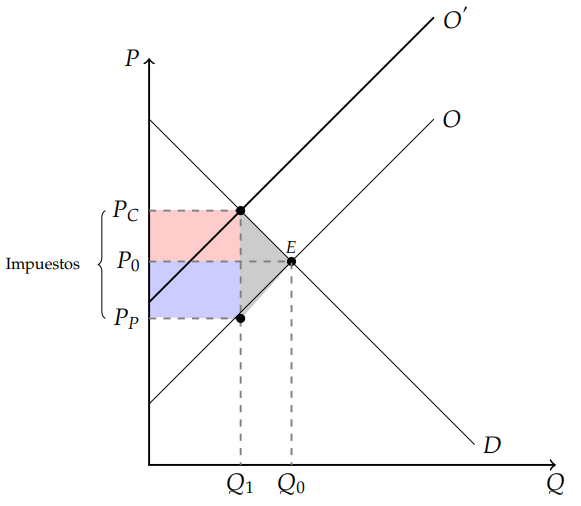
\includegraphics[scale=0.7]{../Figures/C24.4.png}
\end{frame}

\begin{frame}
\frametitle{Veamos un ejemplo}
\begin{itemize}
    \item La demanda es Q = 7000 - 40 P 
    \item La oferta Q = 100 P
    \item El gobierno coloca un impuesto de \$10
\end{itemize}
\end{frame}

\begin{frame}
\frametitle{Y si tengo un subsidio...}

\end{frame}

\end{document}
